\documentclass[12pt]{article}
\usepackage{graphicx}
\usepackage {color}
\usepackage{pdfpages}
\usepackage{float}
\usepackage{changebar}
\usepackage{enumitem,amssymb}
\renewcommand{\familydefault}{\sfdefault}
\usepackage[margin=1.2in]{geometry}
\usepackage{graphicx}
\usepackage{wrapfig}
\usepackage[super]{cite}
\usepackage{subcaption}
\usepackage[table]{xcolor}
\usepackage{amsmath}
\usepackage[sort, numbers]{natbib}
\usepackage{multirow}
\usepackage{tabularx}
\usepackage{siunitx}
\usepackage{matlab-prettifier}
%%%%%%%%%%%%Defining the margins %%%%%%%%%%%%%%%%%%%%%
\textheight 9.in
\textwidth 6.5in
\topmargin -.5in
\oddsidemargin 0in
\setlength{\parskip}{\smallskipamount}

%%%%%%%%%%%%%%Specific Commands %%%%%%%%%%%%%%%%%%
\newcommand{\eg}{{\em e.g.,}}
\newcommand{\ie}{{\em i.e.,}}
\newcommand{\etc}{{\em etc.,}}
\newcommand{\etal}{{\em et al.}}
\newcommand{\degrees}{{$^{\circ}$}}
\newcommand{\fig}[1]{\textbf{Figure #1}}

%%%%%%%%%%%%%%%%%%%%%%%%%%%% Setting to control figure placement
% These determine the rules used to place floating objects like figures 
% They are only guides, but read the manual to see the effect of each.
\renewcommand{\topfraction}{.9}
\renewcommand{\bottomfraction}{.9}
\renewcommand{\textfraction}{.1}
\renewcommand{\familydefault}{\sfdefault} %setting the san serif font

%%%%%%%%%%%%%%%%%%%%%%%% Line spacing
% Use the following command for ``double'' spacing
%\setlength{\baselineskip}{1.2\baselineskip}
% and this one for an acceptable NIH spacing of 6lpi based on 11pt
%\setlength{\baselineskip}{.9\baselineskip}
% The baselineskip does not appear to work when we include a maketitle
% command in the main file.  Something there must set the line spacing
% If we use this next command, then things seem to work.
\renewcommand{\baselinestretch}{.9}

\setcounter{secnumdepth}{0} %make no numbers but have a table of contents


\begin{document}

\title{HW 2: Medical Imaging Systems}
\author{Jake Bergquist, u6010393 }
\maketitle

\section{Q1}\
a)

b) at the given dimensions, each voxel would have dimensions of $24/192 cmx 24/192 cmx 1.0mm = 1.25 mm x 1.25 mm x 1.0 mm$ giving us a volume of $1.6 mm^3$ per voxel. $85\%$ of this volume is occupied by water in our tumor. Water has a density of $~1 g/cm^3 = 0.001 g/mm^3$ giving us $1.6 mm^3 * 85\% * 0.001g/mm^3 = 0.0014 g$ of water. At an atomic mass of 14 g/mole, at at a mass of 0.0014 g this gives us $\frac{0.0014 g}{14 g/mole} = 0.0001 mole$ of water molecules. At 2 hydrogen per water molecule this gives us a total of $0.0002 mole$ of hydrogen atoms or $1.2 * 10^{21} $ hydrogen nucli in water molecules. Assuming a body temperature of 310.15 K (37 Celsius), knowing that $\gamma/2*\pi = 42.58 MHz/T$ for hydrogen nuclei, with a 3 T magnet:\\ $M_0 = \frac{N\gamma^2h^2}{16\pi^2kT}B_0 =\frac{Nh^2}{4kT}\frac{\gamma^2}{4\pi^2}B_0 = \frac{1.2*10^{21}* (6.6*10^{-34} J/s)^2}{4*(1.4*10^{-23} J/K)*310.15 K}(42.58 MHz/T)^2*3T$


\section{Q2}




\begin{lstlisting}[style=Matlab-editor]
%%
%Problem 5

%kernal a
averaging_kernal = ones(3,3)/9;

%kernal b
%orientation flipped due to matlab conventions
vertical_edge_detector = zeros(3,3);
vertical_edge_detector(:,3) = 1;
vertical_edge_detector(:,1) = -1;

%kernal c
%orientation flipped due to matlab conventions
horizontal_edge_detector = zeros(3,3);
horizontal_edge_detector(1,:) = 1;
horizontal_edge_detector(3,:) = -1;

conv1_results = ...
conv2(MRI_Image,averaging_kernal,'same');
%I use the same argument to not get increased image size
%It does however leave in zero padded edges in the calculation but the
%edges are all background and I do not mind as much there

conv2_results = ...
conv2(MRI_Image,vertical_edge_detector,'same');

conv3_results = ...
conv2(MRI_Image,horizontal_edge_detector,'same');

figure(1);
subplot(2,2,1);
imagesc(MRI_Image')
axis('equal')
axis('tight')
colormap(gray);
title('Original')
subplot(222);
imagesc(conv1_results')
axis('equal')
axis('tight')
colormap(gray);
title('3x3 Average')
subplot(223);
imagesc(conv2_results')
axis('equal')
axis('tight')
colormap(gray);
title('Vertical edge detector')
subplot(224);
imagesc(conv3_results')
axis('equal')
axis('tight')
colormap(gray);
title('Horizontal edge detector')

\end{lstlisting}

%%%%%%%%%%%%%%%%%% Correct Bibliography Style




\end{document}

\begin{figure}[H]
	\centering
	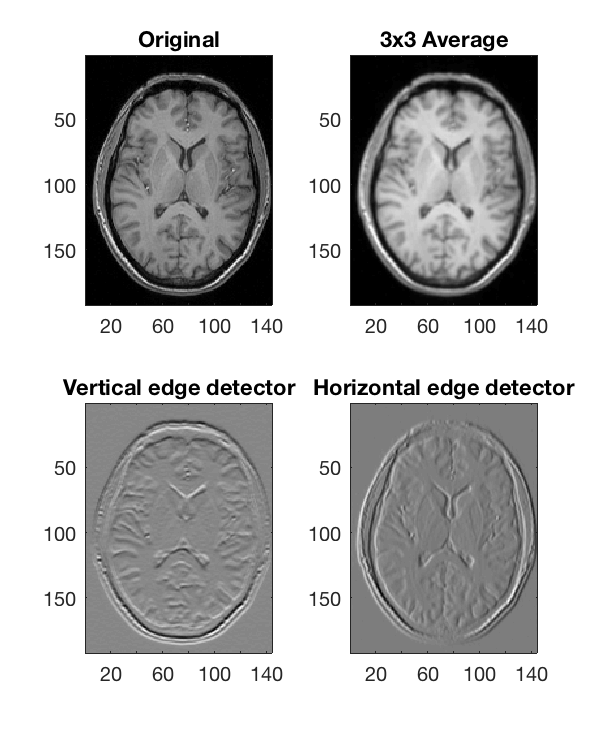
\includegraphics[width=\textwidth]{Figures/convs.png}
	\caption{}
	\label{Fig:conv}
\end{figure}






